\documentclass[sigconf,review]{acmart}

\acmConference[ICSE 2026]{48th International Conference on Software Engineering}{April 2026}{Rio de Janeiro, Brazil}

    
\begin{document}

\title{TrustSECO: a tool for Providing Trust in the Software Ecosystem}


\author{Fang Hou}
\orcid{0000-0002-8042-3278}
\affiliation{%
  \institution{Utrecht University}
  \city{Utrecht}
  \country{Netherlands}
}
\email{f.hou@uu.nl}

\author{Martijn Voordouw}
\affiliation{%
  \institution{Utrecht University}
  \city{Utrecht}
  \country{Netherlands}
}
\email{m.n.voordouw@uu.nl}


\author{Slinger Jansen}
\orcid{0000-0003-3752-2868}
\affiliation{%
  \institution{Utrecht University}
  \city{Utrecht}
  \country{Netherlands}
}
\affiliation{%
  \institution{Lappeenranta University of Technology}
  \city{Lahti}
  \country{Finland}}
\email{slinger.jansen@uu.nl}


            
%
\begin{abstract}


The software ecosystem is a trust-rich part of the world. Software engineers trust major hubs in the ecosystem, such as package managers, repositories, and programming language communities. However, recent increases in software supply chain attacks demonstrate that such trust is often assumed rather than verified. To address this gap, we introduce TrustSECO, a community-managed infrastructure that collects trust-related data, scans software components, and generates trust scores for them. TrustSECO integrates data from multiple sources, such as GitHub, Libraries.io, Stack Overflow, Common Vulnerabilities and Exposures~(CVE), and ClamAV. It aggregates them into transparent trust scores using empirically derived weights. The scores enable software engineers, security professionals, and end-users to assess the reliability, security, and health of software packages. We present the design of TrustSECO, detail its trust score methodology, and report on an evaluation involving 20 industry practitioners who assessed its practical value in software package selection. Results indicate that TrustSECO improves practitioners’ awareness of software risks and supports more deliberate decision-making.


\end{abstract}
%
\keywords{Software Trust, Software Selection, Software Engineering}

%Two concepts need to be explained: (1) Trust Scores and (2) the decentralized aspect

%The screens we have are:

%Home - Shaming and Praising screen

%Trust Scores - What do we collect

%Trust Score Calculation - How do we calculate

%Job List 

%Metrics

\maketitle  

\section{Introduction}
The worldwide Software Ecosystem (SECO) concerns all software-producing and consuming individuals and organizations, which collaboratively ensure that our society remains functional. Throughout the software life cycle, software engineers, end-users, and other stakeholders collaboratively place their trust in major hubs in the ecosystem, such as package managers, repository services, and software components. Trust is a critical factor influencing the acceptance and effective use of technologies, especially in assisting software end-users in mitigating the risks and uncertainties when adopting any uninformed or new technology~\cite{pavlou2002institution}. 

%In our previous systematic literature review, we defined software trust as ``\textit{the willingness of SECO actors to accept risks based on subjective beliefs. It is essentially an upstream trust in that actors expect assurance that other actors on top of a common technology platform can exhibit reliable behavior and provide valuable software products}''. Jensen et al.~\cite{jensen2018codetrust} argue that establishing trustworthiness in software often involves factors like security, reliability, and maintainability.

Trust in SECOs is compromised, it undermines the integrity and reliability of software systems~\citep{hatcliff2014certifiably}. The trust erosion affects secure transactions, data privacy, and system dependability~\citep{pearson2010privacy}. However, based on the software supply chain report~\cite{Sonatype2024OSS}, in 2024, over 512,847 malicious packages were logged in, marking a 156\% increase year-over-year; 92\% of crowdsourced or publicly available data required corrections; only 10.5\% of the open-source packages were actively chosen. It emphasizes that facts influencing the health of software supply chains are largely determined by a selection of open-source components. 

To address trust challenges and restore confidence in SECOs, and to help software practitioners better understand component information and safely select trustworthy components, we design and implement TrustSECO, a community-managed infrastructure that continuously collects and discloses trust facts about software packages, leveraging distributed ledger technology to ensure transparency and immutability. A trust score is introduced that aggregates heterogeneous data sources (e.g., GitHub, Libraries.io, Stack Overflow, CVE, and ClamAV) using empirically derived weights refined through practitioner interviews. The framework is shown in Figure~\ref{fig:npmSECO}. This tool is specific for software engineers, who are deciding which software packages to include in their work, security OPS, who are deciding which software to allow in working configurations in large organizations, and end-users who need trustworthy software. Additionally, we invite 20 industry practitioners to assess the trust data presentation and score calculation of this tool. Results show that TrustSECO improves awareness of software risks and influences package selection practices.

%%%%%%%%%%%%%%%%%%%%%%%%%%%%%%%%%%%%%%%%%%%%%%%
\section{Related Work}
\label{sec2:related}

We conducted a set of research on trust in SECOs to examine both the conceptual foundations of trust and its practical role in software selection. Prior studies have highlighted that trust arises from a combination of technical, organizational, and structural assurance facts, influencing how practitioners adopt open-source and closed-source software. Our systematic literature review has emphasized the importance of security, reliability, and maintainability as central to software trustworthiness~\cite{hou2023systematic}. A set of interviews with 24 practitioners further reveals that software selection is not purely technical but shaped by organizational priorities and perceptions of risk~\cite{hou2023role}.

In practice, several tools and services provide partial support for assessing the trustworthiness of software packages. For example, Snyk, OSS Review Toolkit, and Dependency-Track focus primarily on detecting vulnerabilities and license risks. Similarly, Libraries.io and GitHub metrics expose metadata such as dependencies, GitHub Stars, or the number of contributors, but do not provide a comprehensive trust model. These approaches offer valuable insights but remain fragmented, focusing narrowly on security vulnerabilities or surface-level popularity metrics without synthesizing them into a holistic, empirically validated assessment of trust.

TrustSECO differs in three ways. First, it introduces a community-managed infrastructure underpinned by distributed ledger technology (DLT), ensuring transparency and immutability of collected trust facts. Second, it not only aggregates various data sources into scores of Community and Popularity, Dependencies and Ecosystem, Project Health and Maintenance, and Security, but also consolidates them into a single trust score. Third, the weighting of trust facts is empirically grounded through both large-scale data analysis and practitioner interviews. 

%%%%%%%%%%%%%%%%%%%%%%%%%%%%%%%%%%%%%%%%%

\section{Design of the Tool}
\label{sec3:tool}

TrustSECO is a community-managed infrastructure that underpins the SECO with a trust layer. All the trust facts mined by the members (different stakeholders who participate in the network) will be sourced to the DL. Trust facts can be collected from various data sources. Subsequently, when members and users specify a particular software~(version) through the TrustSECO web-based portal, it retrieves the corresponding trust facts from the DL. Based on our trust score calculation mechanism, they are able to establish whether a particular version of a package can be trusted. Ecosystem hubs can reuse the data from the DL directly. For instance, we have integrated it into npm, a well-known software package manager in another work~\cite{hou2024npmseco}. Software engineers can get the trust-related information of the specific package and its dependencies before the installation. It can also scan all the installed packages for the trust assessments. In cases where trust facts do not exist in the database, TrustSECO proactively acquires the facts from the sources and calculates the trust score. Figures~\ref{fig:screenshot1},~\ref{fig:screenshot2}, and~\ref{fig:screenshot3} display the Trust Score results for package {$requests$} version 2.32.3 on the TrustSECO website~\footnote{\hyperlink{https://trustseco1.science.uu.nl/}{https://trustseco1.science.uu.nl/}}. 


\begin{figure}[!ht]
    \centering
    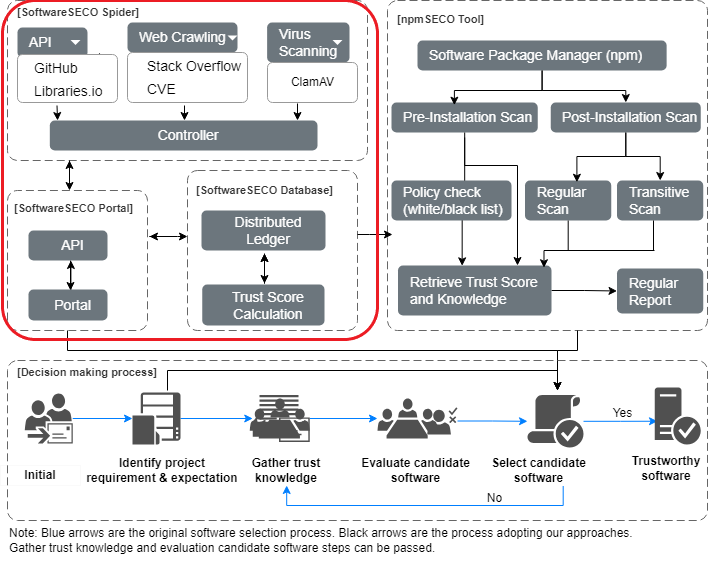
\includegraphics[width=0.5\textwidth]{images/trustseco framework.png} 
    \caption{Overview of the TrustSECO framework. In this paper, we mainly present the red block part. The block of npmSECO Tool is the implementation of TrustSECO in npm.}
    \label{fig:npmSECO}
\end{figure}

%\vspace{-1em}


TrustSECO encourages users to add packages or mine jobs. The TrustSECO infrastructure has two tasks: a spider is exploring the software packages and finding trust facts. These trust facts are observed by different spiders to obtain a consensus on these observations. Once consensus is reached, the observed trust fact is stored in an immutable data structure, i.e., the TrustSECO DL.

The Controller parses the JSON input to send the appropriate commands to the various data sources. APIs are adopted to collect the data from the sources that have existing REST API, for instance, GitHub and Libraries.io. Web crawling is used for any data source that does not provide an API, e.g., the CVE database, or for facts that are not exposed by an API, e.g., GitHub’s user count. We also employ ClamAV, which is an open-source anti-virus toolkit. Through the UNIX socket, a file or file-stream can be given to the ClamAV scanner. The ClamAV scanner searches for any viruses within this file or stream. %A UNIX socket stream pass-through is used, as this eliminates the need for the files to be saved to disk.

Trust-related data includes package basic information, such as the package name, version, platform, owner, language, linkage of the repository, trust score, and trust facts. The trust facts are divided into four categories, namely Community and Popularity, Dependencies and Ecosystem, Project Health and Maintenance, and Security. The trust facts, shown in Table~\ref{tab:npm-factor}, are informed by the existing literature, including GitHub~(development activity), Libraries.io~(dependency risk), Stack Overflow~(community trust), CVE~(security vulnerabilities), and ClamAV~(virus Detection). CVE serves as a repository of publicly disclosed vulnerabilities. It is the most influential vulnerability database~\cite{sun2022heterogeneous}. 


The trust fact weights are based on the study~\cite{mujahid2023characteristics}. This study conducts a quantitative analysis of the selection facts based on a set of 2,527 npm packages, subsequently establishing a ranking based on these facts. We engaged 24 software engineers to discuss the facts influencing their package selection~\cite{hou2023role}. Their insights were used to refine and adjust this ranking. Finally, we incorporated this enhanced rank to determine the relative contribution of each fact.


%An example of how TrustSECO works is illustrated by an example with the Node Package Manager (npm). When a software engineer is developing software and including existing npm components, she might download them through npm. TrustSECO can be used to provide warnings about particular configurations. TrustSECO, before downloading and installing a package, can, for instance, automatically advise the software engineer on the trust rating of the package. If the package (version) is below a particular rating set by the software engineer's organization, npm can use TrustSECO to select another version of the package or even a wholly different package. Furthermore, TrustSECO can warn the software engineers when any new vulnerabilities arise in one of the installed packages. 

\begin{figure}[!htbp]
    \centering
    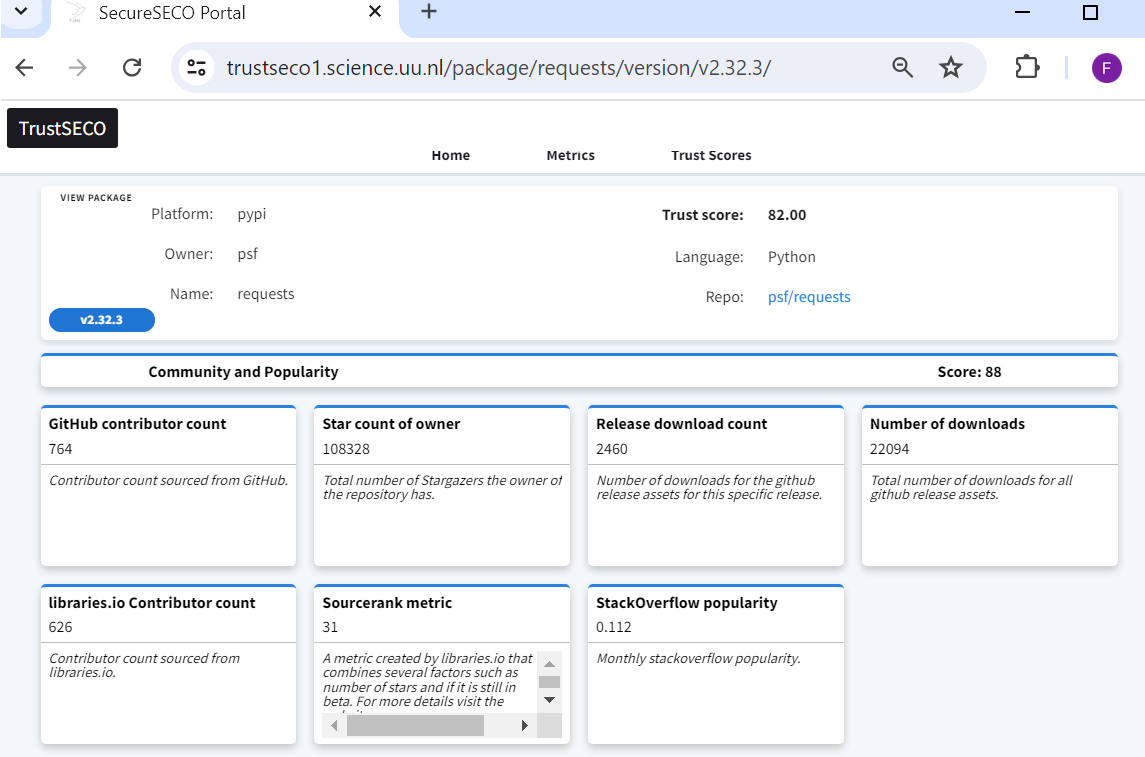
\includegraphics[width=0.48\textwidth]{images/Screenshot_Community and Popularity.PNG}
    \caption{Basic information and details of Community and Popularity for package {$requests$} version 2.32.3 on TrustSECO website.}
    \label{fig:screenshot1}
\end{figure}

\begin{figure}[htbp]
    \centering
    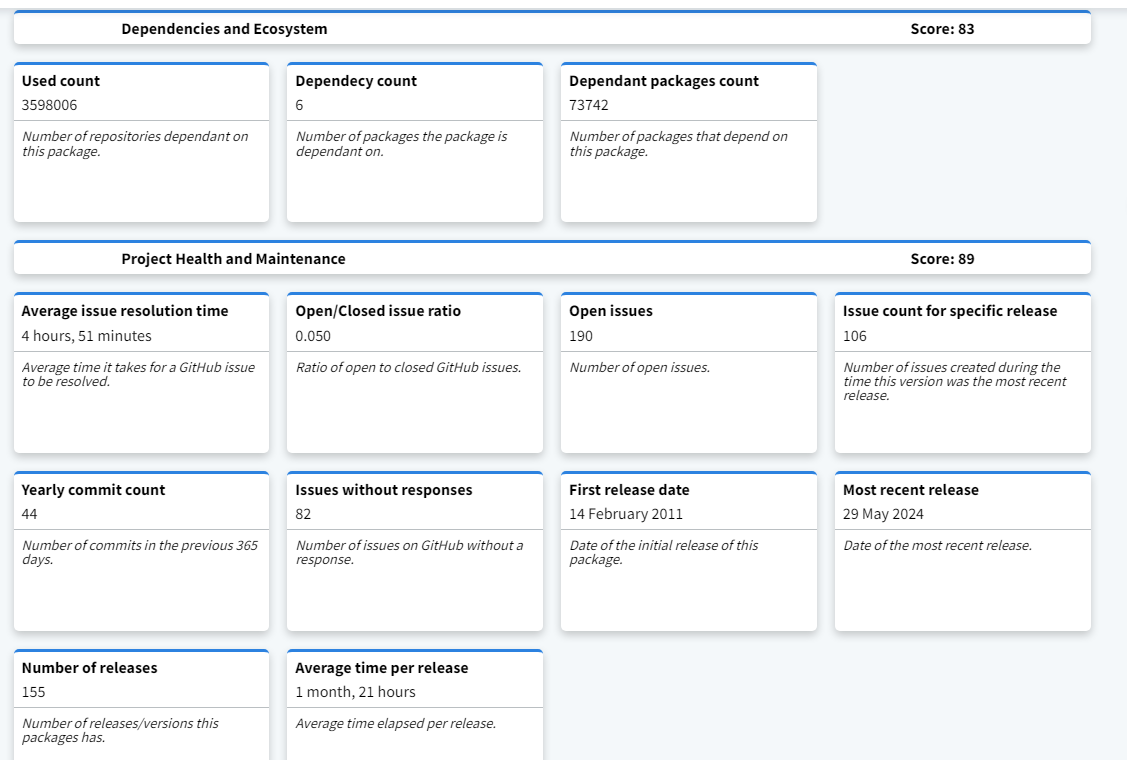
\includegraphics[width=0.48\textwidth]{images/Screenthos_dependency and Project health.PNG}
    \caption{Details of Dependencies and Ecosystem, and Project Health and Maintenance for package {$requests$} version 2.32.3 on TrustSECO website.}
    \label{fig:screenshot2}
\end{figure}

\begin{figure}[!htbp]
    \centering
    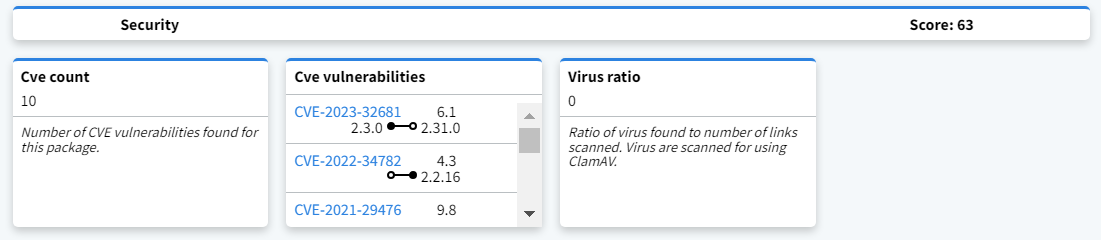
\includegraphics[width=0.48\textwidth]{images/Screenthos_security.PNG}
    \caption{Details of Security for package {$requests$} version 2.32.3 on TrustSECO website.}
    \label{fig:screenshot3}
\end{figure}

%\vspace{-1em}

\begin{table}[!ht]
\centering
\caption{Overview of the Trust facts}
\label{tab:npm-factor}
\resizebox{0.5\textwidth}{!}{%
\small
%\begin{tabular}{@{}p{3cm}p{2cm}p{1cm}p{5cm}@{}}
\begin{tabular}{@{}p{4.5cm}lp{1cm}l@{}}
\toprule
\textbf{Trust Facts} & \textbf{Sources} & \textbf{Weight} & \textbf{Category} \\ \midrule
Number of downloads & GitHub & 63 & Community and Popularity \\
Number of stargazers & GitHub & 24.21 & Community and Popularity  \\
Popularity & Stack Overflow & 18 & Community and Popularity \\
SourceRank & Libraries.io & 8 & Community and Popularity \\
Number of contributors & GitHub & 6 & Community and Popularity \\
Number of contributors & Libraries.io & 4.41 & Community and Popularity \\
Number of downloads per release & GitHub & 1 & Community and Popularity \\
GitHub Stars  & GitHub & 1 & Community and Popularity \\
Number of dependent repositories & Libraries.io & 60 & Dependencies and Ecosystem \\
Number of dependencies & Libraries.io & 8.04 & Dependencies and Ecosystem \\
Number of dependents & Libraries.io & -1 & Dependencies and Ecosystem \\
Number of yearly commits  & GitHub & 15 & Project Health and Maintenance \\
Number of releases  & GitHub & 2 & Project Health and Maintenance \\
Number of open issues & GitHub & 2 & Project Health and Maintenance \\
Number of releases per release & GitHub & 1 & Project Health and Maintenance \\
Release frequency & GitHub & -2.32 & Project Health and Maintenance \\
Average issue resolution time & GitHub & -4 & Project Health and Maintenance \\
Number of issues without response & GitHub & -7 & Project Health and Maintenance \\
Ratio of open issue & GitHub & -15 & Project Health and Maintenance \\
Number of vulnerabilities & CVE & -16.47 & Security \\
Ratio of detected viruses & ClamAV & -16.47 & Security 
\\ \hline
\multicolumn{4}{l}{\textbf{Followings are part of the facts but are not used for score calculation}}\\ \hline

\multicolumn{4}{l}{First release date}     \\
\multicolumn{4}{l}{Most recent release date }   \\
\multicolumn{4}{l}{List of vulnerabilities with linkage and affected version}   \\
 \bottomrule
\end{tabular}%
}
\end{table}
%\vspace{-1em}



The weights assigned to each fact reflect their relative contributions to the overall trust score. Positive weights indicate a positive impact on trustworthiness, while negative weights indicate a detrimental effect on trustworthiness. The trust score is calculated by aggregating the weighted contributions of all relevant trust facts. All the details are shown on the TrustScore Calculation page, as we introduced in the following sections.

\begin{itemize}
    \item \textbf{Normalization of Fact Values:}
Some facts' values vary significantly (e.g., Number of downloads, the value could be from 1 to 1,000,000), logarithmic scaling can compress the range and make the contribution more proportional. For each trust fact, the raw value is normalized using its average value. If the fact is flagged for logarithmic scaling (log: true), the natural logarithm of the value is taken before normalization:
    
For each trust fact, the raw value is normalized using its average value. If the fact is flagged for logarithmic scaling ({log: true}), the natural logarithm of the value is taken before normalization:
\[
\text{factValue} = 
\begin{cases}
\max(\ln(\text{rawValue}), 0) & \text{if log scale is true} \\
\text{rawValue} & \text{otherwise}
\end{cases}
\]



    \item  \textbf{Aggregating Trust Facts into a Score:}

The contribution of each fact to the trust score is calculated as:

\[
\text{Trust Score}_{\text{i}} = \frac{\text{factValue}_{\text{i}} \times \text{weight}_{\text{i}}}{{\text{average}_{\text{i}} \times \text{occurences}_{\text{i}}}}
\]
where:
\begin{itemize}
    \item \(\text{factValue}\) is the value of the i-th fact (possibly transformed by a logarithmic function).
    \item \(\text{weight}\) is the weight of the i-th fact.
    \item \(\text{average}\) is the average value of the i-th fact (used for normalization).
    \item \(\text{occurrences}\) is the number of occurrences of the i-th fact in the package's data.
\end{itemize}

\item \textbf{Score Compression:}

To ensure the trust score falls within an interpretable range (0 to 100), a logistic function is applied:


\[
\text{squashedScore} = 
\frac{100}{1 + e^{-\text{growth\_rate} \times (\text{score} - \text{midpoint})}}
\]

where:
\begin{itemize}
    \item \(\text{score}\) is the sum of trust scores
    \item \(\text{growth\_rate}\) controls the steepness of the logistic curve. It is the growth rate specific to each category.
    \item \(\text{midpoint}\) determines the center of the curve. It is a central value around which the growth rate is applied.
\end{itemize}

\end{itemize}

As members of the TrustSECO ecosystem need to be trusted, we need them to provide GitHub credentials. So the members can download and run an instance locally to add packages or mine jobs. They can check the metrics and the Spider logs on the Metrics page. 

The DLT metrics include the total number of packages in the system, the blockheight within the ledger, and the number of participants joined the ledger. A job list has been provided to assist participants and supporters in determining if the package information is retrieved successfully. A list is provided, with the package name, version, facts, and related bounty for each fact.
%%%%%%%%%%%%%%%%%%%%%%%%%%%%%%%%%%%%%5
\section{Evaluation}
\label{evaluation}

We tested TrustSECO's functionality by mining the trust data of more than 400 software packages (including multiple versions for each package). We invited 20 practitioners (P1 to P20) to evaluate the trust facts and scores presentation on the portal. These practitioners were domain experts from software companies involved in the search for software packages (15 participants indicated a frequency score of 4 or higher, on a scale of the frequency of searching for software packages, 1-5 indicating from ``never'' to ``very often''; mean = 3.85, median = 4, which underscores they are well experienced and expectant about the software package selection). Interview protocol and participant feedback are saved as online materials\footnote{\hyperlink{https://figshare.com/s/4db3d34847d97fd65953}{https://figshare.com/s/4db3d34847d97fd65953}}.

In terms of the provided trust facts and scores, overwhelmingly positive feedback emerges from the surveyed engineers. Specifically, 19 participants believe this feature improved their understanding of the packages they considered, promoting more careful decision-making. According to P9 and P14, by utilizing this tool, they may be aware that it is imperative to exercise caution before installing external libraries, particularly in large projects that may consist of a variety of libraries. P2, P5, and P20 contend that sometimes software engineers overlook details about a package, and trust scores serve as a guide or alert to help prevent such errors from occurring. 

However, some participants point out that trust scores and some facts do not fully reflect the trust of a software package. For instance, P6 highlights that the trust score may introduce an unfair bias towards new packages due to insufficient trust facts. For instance, total downloads, number of software engineers, or frequency of releases, may have low values for new packages, leading to lower trust scores unfairly impacting their evaluation. P10 notes that the trust of a package may not depend on frequent updates. It could be a well-functioning tool that does not require constant changes. Similarly, some facts, such as the number of GitHub Stars, may not always reflect the true value of a library, and a perfectly functioning package does not need to commit anything, so the number of commits per year drops close to zero. Another one is the contributor count. P20 points out that most software engineers could see no reason why the number of people working would affect software trust. Four participants highlight that certain trust facts, such as GitHub Stars, first release date, and contributor count, are redundant or not particularly useful. While understanding the feature's broader appeal, P3, P6, and P20 personally prefer accessing information directly from GitHub or sticking to their existing processes. In addition, two participants propose enhancements to the trust score calculation process. They emphasize the importance of the dependencies, and point out that a package's trust score should not exceed that of its lowest-scoring dependency. 

To further assess this tool, we plan to invite more software practitioners to assess it from seven aspects (including Usability, Data Sources, Trust Score Methodology, Security \& Accuracy, Comparison to Alternatives, Practical Value, and Sustainability), and find a better solution for the scoring methodology to handle new or niche packages and extend TrustSECO to more ecosystems.

%%%%%%%%%%%%%%%%%%%%%%%%%%%%%%%%%%%%%%%%%%%%%
\section{Threats to Validity}
\label{sec5:threat}

\noindent\textbf{Internal validity}: Participants may have been influenced by their facts and package selection practices. To mitigate this, we selected practitioners with diverse backgrounds, and we plan to involve more practitioners to assess it.

\noindent\textbf{Construct validity}: The trust score may not fully capture all aspects of “trust” as understood by practitioners. Certain facts (e.g., GitHub stars or contributor counts) were considered less meaningful by some participants. While our weighting scheme was refined using empirical data and interviews, future work should investigate alternative scoring models.


%%%%%%%%%%%%%%%%%%%%%%%%%%%%%%%%%%%%%%%%%%%%



\section{Conclusions}
\label{sec6:conclusion}

The contribution of the TrustSECO infrastructure lies in its design, which implements trust scores on software packages and offers comprehensive trust factors. Trust scores allow for the calculation of trustworthiness in complex combinations of software packages and numerical data, facilitating a quick assessment of the software packages. Our initial evaluation with industry practitioners demonstrates that TrustSECO increases awareness of software risks and fosters more careful adoption practices. Future work will conduct larger-scale empirical studies to improve this tool. Our purpose is to form a foundational trust layer for software ecosystems, mitigating risks and enhancing the resilience of modern software supply chains.






%Trust operates under risk and uncertainty~\cite{elster2015explaining}, which means that without risk and uncertainty, there would be no need for trust to exist. 


%Jensen et al.~\cite{jensen2018codetrust} argue that trustworthiness in software is defined as the level of confidence that software will meet its goals while remaining free from threats under all circumstances. Efforts to establish trustworthiness in software often involve parameters like security, reliability, and maintainability.

%According to Nadi et al. \cite{nadi2023selecting}, software package selection is often a difficult task, with considerable factors, such as technical factors, human factors, and economic factors influencing this selection. While many assume that the SECO hub can perform some quality check or trust analysis, it rarely does. Some expose some simple trust knowledge, such as the number of downloads or ``stars'' of appreciation given by the community, but generally, they do not take the responsibility of providing anything more than basic reporting services (``\textit{Report a problem with this package}''). 

%We propose TrustSECO, which is a community-managed infrastructure that underpins the SECO with a trust layer. The infrastructure gathers data on trust in particular software packages and projects. With this data, software end-users can determine whether packages (versions) are reliable, contain vulnerabilities, and are trusted by other users. The purpose is to use empirical software engineering to secure the worldwide SECO. 

\bibliographystyle{splncs04}
\bibliography{Ref}

\end{document}
